Im Folgenden wird, um unnötig viele Indices zu vermeiden, die Zahl der Messungen in einem Zeitintervall $N_{\Delta t}$ mit $N$ bezeichnet. \\
Die Messung des Nulleffekts ergibt einen Offset von
\begin{align}
	N_{u,\text{\ce{Br}}} &= \frac{182}{900}\si{\counts\per\second} = \SI{36.4}{\counts\per\intervall} \\
	N_{u,\text{\ce{Ag}}} &= \frac{222}{1200}\si{\counts\per\second} = \SI{1.85}{\counts\per\intervall} \ .
\end{align}
Dieser wird von den aufgenommenen Werten abgezogen, die dann erhaltenen eigentlichen Zerfallsraten $N$ pro Messintervall inklusive dem statistischen Fehler $\sqrt{N}$, der aus der Poissonverteilung des radioaktiven Zerfalls kommt, sind in Tabelle \ref{Werte} dargestellt.
\begin{table}[h!]
\centering
        \caption{In einem Intervall gemessene Pulse nach Abziehen des Nullwertes}
        \label{tab:Werte}
\begin{tabular}{cccc}
	\toprule
	$N_\text{\ce{Ag}}$ & $\Delta N_\text{\ce{Ag}}$ & $N_\text{\ce{Br}}$ & $\Delta N_\text{\ce{Br}}$ \\
	\midrule
	77  & 9   & 351 & 19 \\
51  & 7   & 290 & 17 \\
50  & 7   & 250 & 16 \\
35  & 6   & 269 & 16 \\
32  & 6   & 241 & 16 \\
27  & 5   & 212 & 15 \\
24  & 5   & 234 & 15 \\
19  & 4   & 227 & 15 \\
13  & 4   & 217 & 15 \\
18  & 4   & 248 & 16 \\
18  & 4   \\
18  & 4   \\
15  & 4   \\
15  & 4   \\
10  & 3   \\
16  & 4   \\
12  & 3   \\
9   & 3   \\
12  & 3   \\
8   & 3   \\
10  & 3   \\
7   & 3   \\
7   & 3   \\
7   & 3   \\
6   & 2   \\
5   & 2   \\
5   & 2   \\
10  & 3   \\
0.1 & 0.4 \\
5   & 2   \\
7   & 3   \\
4   & 2   \\
7   & 3   \\
8   & 3   \\
3   & 2   \\
1   & 1   \\
4   & 2   \\
8   & 3   \\
4   & 2   \\
1   & 1   \\
3   & 2   \\
4   & 2   \\

	\bottomrule
\end{tabular}
\end{table}


\subsection{Brom}
Für den Zerfall von Brom gilt
\begin{align}
	N_{\Delta t}(t) &= N_0\exp(-\lambda t) 
- N_0\exp(-\lambda(t+\Delta t)) 
= N_0\left(1-\exp(-\lambda\Delta t)\right)\exp(-\lambda t) \\
	\Leftrightarrow \ln N_{\Delta t}(t) &= \ln N_0\left(1-\exp(-\lambda\Delta t)\right) \ - \lambda t \ .
\end{align}
\todo{Die Auswertmethode gehört dann nicht in die Theorie?}
Da $\ln N_0\left(1-\exp(-\lambda\Delta t)\right)=const$ gilt kann eine lineare Ausgleichsrechnung mit den Wertepaaren $\{t_i, \ln N_{\Delta t}(t_i)\}$ durchgeführt werden. Der Zeitpunkt $t_i$ ist hierbei der Zeitpunkt nach dem $i$-ten Messintervall (also $t_3 = 3\Delta t=\SI{450}{\second}$). Der Graph der linearen Regression ist in Abbildung \ref{fig:Brom} zu sehen, die Rechnung mit Python berechnet die Parameter (Steigung $m$, Achsenabschnitt $b$)
\begin{align}
	m &= -\lambda = \SI{-0.012+-0.004}{\per\second}
 \\
	b &= \SI{5.72+-0.07}{}
 \ .
\end{align}
Die Halbwertszeit von Brom-80 ist demnach
\begin{align}
	T_\text{\ce{^80_35Br}} = \frac{\ln2}{\lambda} = \SI{57.0}{\second}
 \ .
\end{align}
\begin{figure}[h!]
	\centering
	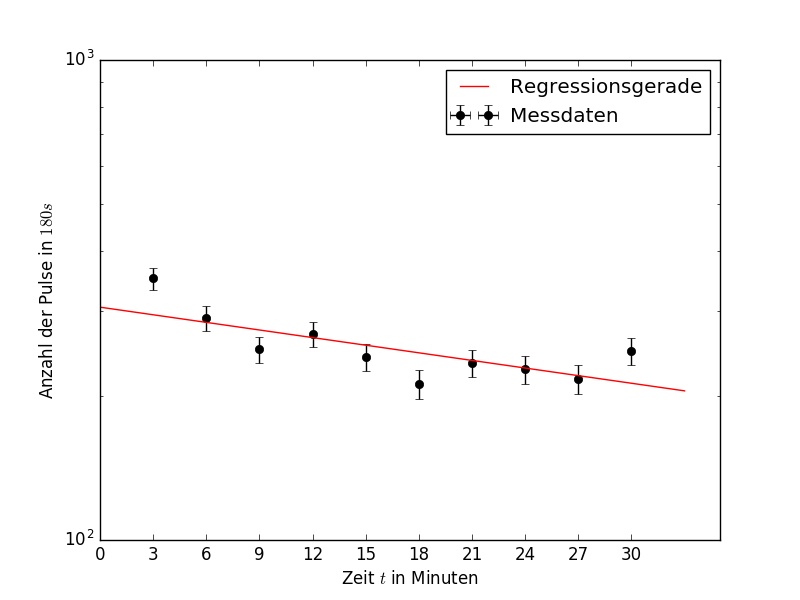
\includegraphics[width=0.7\textwidth]{build/Brom.png}
	\caption{Regressionsgerade Brom}
	\label{fig:Brom}
\end{figure}

\subsection{Silber}
Bei Silber finden zwei Zerfälle statt. Um sie zu Trennen wird ein Punkt bestimmt, ab dem nur noch der lange Zerfall eine Rolle spielt. Es wird $t=\SI{130}{\second}$ gewählt. Mit den Werten rechts davon wird nun eine lineare Regression, wie im vorigen Abschnitt für Brom durchgeführt. Allerdings werden einige Werte (siehe Abbildung \ref{fig:Silber}) nicht berücksichtigt, da sie zu stark abweichen und das Ergebnis verfälschen würden. Die Ausgleichsrechnung liefert hier
\begin{align}
	m &= -\lambda = \SI{-0.0047+-0.0005}{\per\second}
 \\
	b &= \SI{3.1+-0.2}{}
 \ ,
\end{align}
woraus sich eine Halbwertszeit von
\begin{align}
	T_{\text{\ce{^108_47Ag}}} = \SI{146.662+-0.008}{\second}

\end{align}
ergibt. \\
Um die Halbwertszeit für den kurzlebigen Zerfall zu erhalten werden nun die Werte mit $t<\SI{90}{\second}$ gewählt. Der Anteil des langen Zerfalls wird abgezogen, sodass allein der Anteil des kurzen Zerfalls übrig bleibt. Wiederum wird eine lineare Regression durchgeführt, die Parameter lauten
\begin{align}
        m &= -\lambda = \SI{-0.023+-0.002}{\per\second}
 \\
        b &= \SI{4.5+-0.1}{}
 \ ,
\end{align}
die Halbwertszeit lautet
\begin{align}
        T_{\text{\ce{^108_47Ag}}} = \SI{146.662+-0.008}{\second}
 \ .
\end{align}
Abbildung \ref{fig:Silber} zeigt die Regressionsgeraden mit den verwendeten Werten. \\
\begin{figure}[h!]
        \centering
        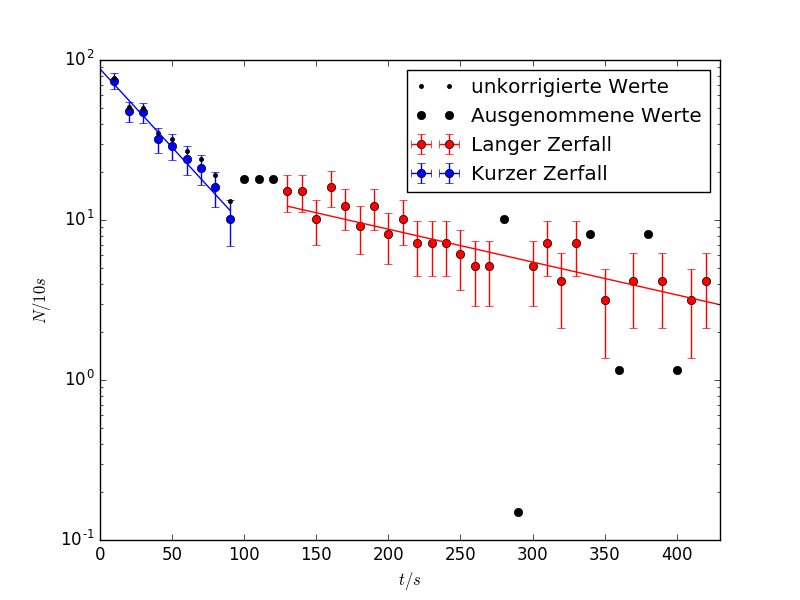
\includegraphics[width=0.7\textwidth]{build/Silber.png}
        \caption{Regressionsgeraden Silber. Für die Regression wurden die Werte des reinen kurzen Zerfalls verwendet. Die Werte, bei denen der lange Zerfall noch nicht abgezogen wurde, werden als unkorrigierte Werte bezeichnet.}
        \label{fig:Silber}
\end{figure}
Der gesamte Zerfall beider Isotope kann durch einfach Addition der beiden Geraden erhalten werden. Dabei ist zu beachten, dass gilt
\begin{align}
N_{\Delta t}(t) &= N_{0,\text{k}}\exp(-\lambda_\text{k} t) + N_{0,\text{l}}\exp(-\lambda_\text{l} t) - N_{0,\text{k}}\exp(-\lambda_\text{k}(t+\Delta t)) + N_{0,\text{l}}\exp(-\lambda_\text{l}(t+\Delta t)) \\
	&= N_{0,\text{k}}\exp(-\lambda_\text{k} t)\left( 1 - \exp(-\lambda_\text{k}\Delta t)\right)
	+ N_{0,\text{l}}\exp(-\lambda_\text{l} t)\left( 1 - \exp(-\lambda_\text{l}\Delta t)\right) \ , 
\end{align}
sodass nicht die Geraden addiert werden, sondern die exponentiellen Zerfallskurven vor dem Logarigthmieren. Die addierten Kurven sind in Abbdildung \ref{fig:addiert} zu sehen.
\begin{figure}[h!]
        \centering
        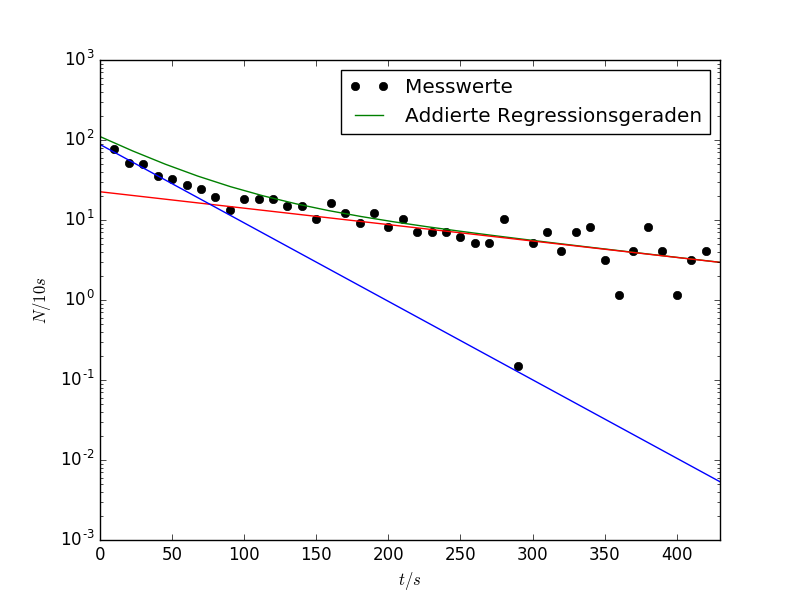
\includegraphics[width=0.7\textwidth]{build/SilberAddiert.png}
        \caption{Addierte Zerfälle bei Silber}
        \label{fig:addiert}
\end{figure}

